%=====================================================================
\section{MILP baseline: how the 560 instances ended}

\begin{figure}[H]
\centering
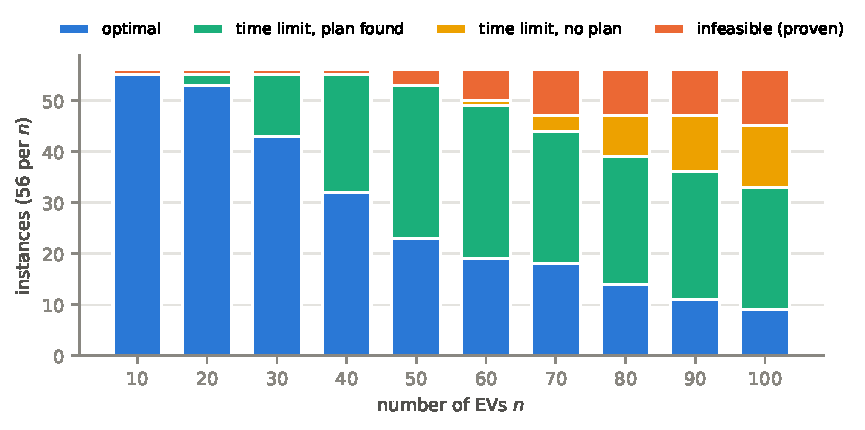
\includegraphics[width=0.88\textwidth]{figures/milp_status_by_n.pdf}
\caption{Result of the MILP for each instance size (56 instances per size).}
\label{fig:status}
\end{figure}

\begin{table}[H]
\centering
\caption{MILP baseline by Solomon class. Median gap: over the time-limited instances with a plan.}
\small
\begin{adjustbox}{max width=\linewidth}
\begin{tabular}{@{}lrrrrrrrrr@{}}
\toprule
class & instances & optimal & time limit & no plan & infeasible & valid & \shortstack{median\\gap (\%)} & \shortstack{mean\\time (s)} & \shortstack{mean $Z$\\(Rs)} \\
\midrule
C1 & 90 & 66 & 23 & 1 & 0 & 89 & 4.1 & 110 & 47470 \\
C2 & 80 & 56 & 23 & 1 & 0 & 79 & 2.9 & 109 & 47996 \\
R1 & 120 & 41 & 34 & 16 & 29 & 75 & 4.4 & 137 & 32677 \\
R2 & 110 & 70 & 40 & 0 & 0 & 110 & 2.6 & 130 & 44782 \\
RC1 & 80 & 13 & 29 & 16 & 22 & 42 & 7.8 & 171 & 36587 \\
RC2 & 80 & 31 & 48 & 1 & 0 & 79 & 2.9 & 189 & 49691 \\
\bottomrule
\end{tabular}
\end{adjustbox}

\end{table}

\begin{itemize}
  \item \textbf{\fmilpOptimal{} instances optimal}, \fmilpTL{} stopped at the time limit with a plan (median gap \fmilpGapMedian\,\%, mean \fmilpGapMean\,\%), \fmilpTLnoPlan{} stopped \emph{without} a plan, \fmilpInfeasible{} proven infeasible. In total \fmilpValid{} valid plans. Mean solve time \fmilpSolveMean{} s.
  \item \textbf{Size decides difficulty.} Up to 20 cars almost everything is optimal in seconds. From about 50 cars, most instances hit the 300-second limit.
  \item \textbf{The infeasible and unsolved instances are in R1 and RC1}, the classes with very short periods (230--240 min). There 100 cars, many requesting late, cannot all be charged by $T$ with 24 guns and 5 vans. The 51 infeasible instances are exactly the 51 of formulation 3: infeasibility comes from the data (time, range, fleet), not from the customer numbers.
  \item The greedy rule alone finds a valid plan in \fgreedyValid{} instances; the MILP starts from that plan and finds valid plans in 13 more instances.
  \item Compared with formulation 3 (same data, one customer type), formulation 4 proves more instances optimal (277 against 256); the other statuses are almost unchanged.
\end{itemize}

\inshort{The MILP solves small instances to optimality and large ones to within a few per cent; the only failures are the short-period classes R1 and RC1 at 60--100 cars, mostly because no plan can exist there.}

%=====================================================================
\section{MILP baseline: what the cost is made of}
\label{sec:anatomy}

\begin{table}[H]
\centering
\caption{The six parts of $Z$, over the \fmilpValid{} valid MILP plans.}
\small
\begin{adjustbox}{max width=\linewidth}
\begin{tabular}{@{}lrr@{}}
\toprule
term & mean per instance (Rs) & share of $Z$ (\%) \\
\midrule
$Z_1$ EV driving (perceived) & 388 & 0.9 \\
$Z_2$ van driving & 1067 & 2.4 \\
$Z_3$ van dispatch & 3291 & 7.5 \\
$Z_4$ operator energy & 9204 & 20.9 \\
$Z_5$ tariff (perceived) & 17310 & 39.3 \\
$Z_6$ time (perceived) & 12739 & 29.0 \\
\midrule
$Z$ (all six) & 43999 & 100.0 \\
\bottomrule
\end{tabular}
\end{adjustbox}

\end{table}

\begin{itemize}
  \item \textbf{The tariff felt by customers ($Z_5$) is the largest part} (\fshareZFive\,\%): every car pays for 10--40 kWh, and most customers are poor commercial drivers who feel each rupee strongly.
  \item \textbf{Customers' time ($Z_6$) is next} (\fshareZSix\,\%): about an hour per car from request to full charge.
  \item \textbf{The operator's energy ($Z_4$)} is \fshareZFour\,\%; van dispatch \fshareZThree\,\%; van driving and EV driving are small.
\end{itemize}

\inshort{Two thirds of $Z$ is what customers feel (money and time); a third is the operator's cost, mostly electricity.}

%=====================================================================
\section{MILP baseline: who gets a van}

\begin{table}[H]
\centering
\caption{The two segments in the baseline plans of the MILP and of RL (RL is discussed in Part V). Free-choice cars have a station within range. Note: the MILP and RL columns are over their own valid plans (\fmilpValid{} and \frlValid{} instances).}
\small
\begin{adjustbox}{max width=\linewidth}
\begin{tabular}{@{}lrrrr@{}}
\toprule
 & personal MILP & personal RL & commercial MILP & commercial RL \\
\midrule
EVs in valid plans & 7043 & 7768 & 16787 & 18282 \\
free-choice EVs & 6095 & 6727 & 14125 & 15418 \\
van share of free-choice EVs (\%) & 19.9 & 6.7 & 0.7 & 0.9 \\
mean $\theta$ & 0.69 & 0.69 & 0.36 & 0.36 \\
mean queue at FCS (min) & 0.41 & 0.79 & 1.58 & 3.36 \\
mean wait for a van (min) & 19.8 & 21.8 & 24.5 & 28.3 \\
mean drive to FCS (min) & 7.8 & 8.3 & 8.9 & 11.3 \\
mean time until charged (min) & 60.6 & 61.8 & 64.3 & 68.3 \\
mean money paid (Rs) & 352 & 332 & 335 & 337 \\
mean time cost (Rs) & 381 & 430 & 200 & 214 \\
mean perceived cost (Rs) & 662 & 699 & 582 & 597 \\
\bottomrule
\end{tabular}
\end{adjustbox}

\end{table}

\begin{figure}[H]
\centering
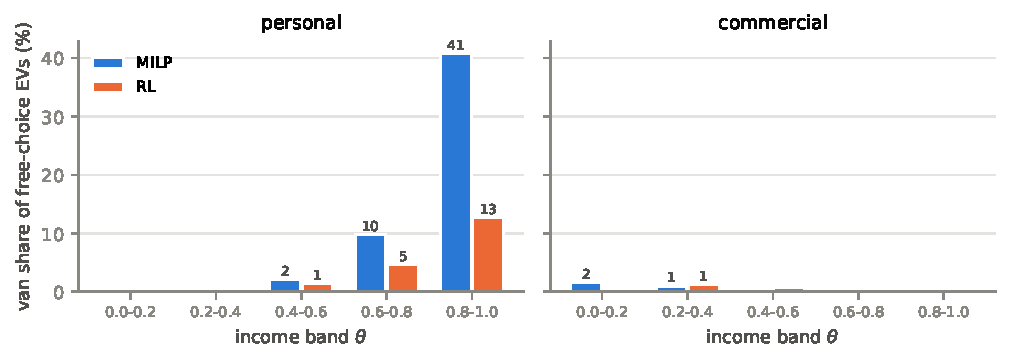
\includegraphics[width=0.95\textwidth]{figures/van_share_income.pdf}
\caption{Share of free-choice cars served by a van, by segment and income band (numbers above the bars in \%).}
\label{fig:vanincome}
\end{figure}

\begin{table}[H]
\centering
\caption{By income band (MILP, all valid plans; van share also for RL). ``Money felt'' is the money paid times the customer's $\mu$.}
\footnotesize
\begin{adjustbox}{max width=\linewidth}
\begin{tabular}{@{}llrrrrrrr@{}}
\toprule
segment & \shortstack{$\theta$\\band} & EVs & van \% MILP & van \% RL & queue (min) & \shortstack{money\\felt (Rs)} & \shortstack{time cost\\(Rs)} & \shortstack{perceived\\cost (Rs)} \\
\midrule
personal & 0.0-0.2 & 125 & 0.0 & 0.0 & 1.45 & 389 & 120 & 509 \\
 & 0.2-0.4 & 690 & 0.0 & 0.0 & 1.32 & 403 & 243 & 646 \\
 & 0.4-0.6 & 1491 & 2.1 & 1.4 & 0.57 & 338 & 337 & 675 \\
 & 0.6-0.8 & 1934 & 9.8 & 4.7 & 0.18 & 263 & 428 & 691 \\
 & 0.8-1.0 & 2803 & 40.8 & 12.7 & 0.06 & 228 & 418 & 646 \\
\midrule
commercial & 0.0-0.2 & 2532 & 1.6 & 0.5 & 2.77 & 457 & 151 & 607 \\
 & 0.2-0.4 & 7633 & 1.0 & 1.3 & 1.76 & 408 & 186 & 594 \\
 & 0.4-0.6 & 5356 & 0.1 & 0.7 & 0.92 & 333 & 226 & 560 \\
 & 0.6-0.8 & 1186 & 0.0 & 0.5 & 0.75 & 286 & 273 & 559 \\
 & 0.8-1.0 & 80 & 0.0 & 0.0 & 0.00 & 167 & 258 & 425 \\
\bottomrule
\end{tabular}
\end{adjustbox}

\end{table}

What the MILP plans show:
\begin{enumerate}
  \item \textbf{Vans go to personal cars.} \fvanPersMilp\,\% of free-choice personal cars get a van, against \fvanComMilp\,\% of commercial cars. This is theory point 3: the driver-free benefit belongs to private owners.
  \item \textbf{Among personal cars, van use rises steeply with income}: 0\,\% below $\theta=0.4$, 2\,\% at 0.4--0.6, 10\,\% at 0.6--0.8, 41\,\% above 0.8. A logistic fit of ``van or not'' on $\theta$ puts the income threshold for personal cars at $\theta^*\approx\fthetaStarPers$: only the very richest are more likely than not to get a van. For commercial cars there is no threshold in $[0,1]$.
  \item \textbf{The few commercial cars with a van are the poorest drivers}, not the richest (1.6\,\% below $\theta=0.2$, 0\,\% above 0.6). They are also the ones with the longest station queues (2.8 minutes on average in the lowest band, 0 in the highest). This is theory point 2: \emph{queues, not income, push taxis to vans}.
  \item \textbf{Commercial cars wait more at stations} (\fqueueComMilp{} against \fqueuePersMilp{} minutes on average) and take longer until charged (64 against 61 minutes). Low-income customers absorb the queues, as theory point 5 predicts.
  \item \textbf{Money paid is about the same in both segments} (about Rs 335--350), but \textbf{money felt} is much higher for commercial drivers (Rs 382 against 281), because they are poorer. Personal owners instead lose more in \emph{time} value (Rs 381 against 200).
  \item By class, the personal van share is lowest in R1 (12\,\%: very short period, a van can make few trips) and highest in RC2 (26\,\%).
\end{enumerate}

\inshort{In the best plans, vans are a service for rich private owners; taxis and poorer customers use the stations and absorb the queues. The rare taxi with a van is a poor driver escaping a long queue.}

%=====================================================================
\section{MILP experiments, one by one}
\label{sec:milpexp}

Each table below shows the MILP row first and then the two RL rows (discussed in Part V). Columns: valid plans; paired instances; instances \emph{new}ly valid or \emph{lost} against the baseline; mean change of $Z$, of the operator's cost and of the customers' cost (paired instances); van share of free-choice cars, baseline $\to$ variant; average number of vans used; for RL the mean gap to the MILP of the same variant.

\subsection{E5: value of charging time}

\begin{table}[H]
\centering
\caption{E5. Value of a station minute for the richest private owner ($c^{C,1}$), and the commercial downtime rate at the top income ($\omega^1$), $\pm25$\,\%.}
\scriptsize
\begin{adjustbox}{max width=\linewidth}
\begin{tabular}{@{}lrrrrrrrrrrr@{}}
\toprule
method & valid & paired & new & lost & \shortstack{$\Delta Z$\\\%} & \shortstack{$\Delta$\\oper. \%} & \shortstack{$\Delta$\\cust. \%} & \shortstack{van \%\\personal} & van \% comm. & vans used & \shortstack{gap to\\MILP \%} \\
\midrule
\multicolumn{12}{@{}l}{\textbf{E5\_cC1\_personal\_7.5}: personal $c^{C,1}$ = 7.5 ($-$25 \%)} \\
MILP & 473 & 472 & 1 & 2 & $-$2.21 & $-$1.15 & $-$2.59 & 19.9 $\to$ 14.1 & 0.7 $\to$ 0.8 & 2.13 & -- \\
RL zero-shot & 499 & 499 & 0 & 1 & $-$2.49 & $-$0.21 & $-$3.45 & 6.7 $\to$ 5.5 & 0.9 $\to$ 0.9 & 2.20 & 0.56 \\
RL retrained & 500 & 499 & 1 & 1 & $-$2.46 & $-$0.59 & $-$3.24 & 6.7 $\to$ 3.9 & 0.9 $\to$ 0.8 & 2.19 & 0.56 \\
\multicolumn{12}{@{}l}{\textbf{E5\_cC1\_personal\_12.5}: personal $c^{C,1}$ = 12.5 ($+$25 \%)} \\
MILP & 473 & 472 & 1 & 2 & $+$2.08 & $+$2.75 & $+$1.84 & 19.9 $\to$ 29.4 & 0.7 $\to$ 0.7 & 2.37 & -- \\
RL zero-shot & 502 & 500 & 2 & 0 & $+$2.45 & $+$0.32 & $+$3.37 & 6.7 $\to$ 8.0 & 0.9 $\to$ 0.8 & 2.23 & 1.22 \\
RL retrained & 500 & 500 & 0 & 0 & $+$2.38 & $+$0.93 & $+$3.02 & 6.7 $\to$ 11.7 & 0.9 $\to$ 0.6 & 2.26 & 1.14 \\
\multicolumn{12}{@{}l}{\textbf{E5\_omega1\_commercial\_4.5}: commercial downtime rate at $\theta=1$: 4.5 ($-$25 \%)} \\
MILP & 472 & 471 & 1 & 3 & $-$2.67 & $-$0.17 & $-$3.80 & 19.9 $\to$ 19.6 & 0.7 $\to$ 0.7 & 2.17 & -- \\
RL zero-shot & 500 & 499 & 1 & 1 & $-$2.72 & $-$0.13 & $-$3.86 & 6.7 $\to$ 6.5 & 0.9 $\to$ 0.8 & 2.19 & 0.82 \\
RL retrained & 500 & 499 & 1 & 1 & $-$2.52 & $+$0.17 & $-$3.69 & 6.7 $\to$ 7.6 & 0.9 $\to$ 0.6 & 2.23 & 0.98 \\
\multicolumn{12}{@{}l}{\textbf{E5\_omega1\_commercial\_7.5}: commercial downtime rate at $\theta=1$: 7.5 ($+$25 \%)} \\
MILP & 475 & 472 & 3 & 2 & $+$2.66 & $+$0.26 & $+$3.81 & 19.9 $\to$ 19.6 & 0.7 $\to$ 0.7 & 2.20 & -- \\
RL zero-shot & 500 & 500 & 0 & 0 & $+$2.72 & $+$0.26 & $+$3.82 & 6.7 $\to$ 6.9 & 0.9 $\to$ 0.9 & 2.24 & 0.83 \\
RL retrained & 499 & 499 & 0 & 1 & $+$2.75 & $+$0.14 & $+$3.92 & 6.7 $\to$ 7.0 & 0.9 $\to$ 0.8 & 2.22 & 0.86 \\
\bottomrule
\end{tabular}
\end{adjustbox}

\end{table}

\begin{itemize}
  \item \textbf{Personal $c^{C,1}$} moves $Z$ by $-2.2$\,\% / $+2.1$\,\% and \textbf{strongly moves the personal van share}: 19.9\,\% $\to$ 14.1\,\% when station time is valued less, $\to$ 29.4\,\% when it is valued more. When rich owners hate station time more, more of them get vans, and the operator pays for it (operator cost $+2.75$\,\%).
  \item \textbf{Commercial $\omega^1$} moves $Z$ by $\mp2.7$\,\% but \textbf{does not change who gets vans} (personal 19.6\,\%, commercial 0.7\,\% in both variants). A taxi's drive, charge and van minutes all scale with $\omega$, so both options become dearer together; only the customers' cost changes ($\pm3.8$\,\%).
  \item Both results are what theory predicted for E5.
\end{itemize}

\inshort{How much private owners hate station time decides how many vans they get; the taxi downtime rate changes the cost but not the choices.}

\subsection{E6: money sensitivity}

\begin{table}[H]
\centering
\caption{E6. How strongly the poorest customer feels a rupee ($\mu^0$), per segment, $\pm25$\,\%.}
\scriptsize
\begin{adjustbox}{max width=\linewidth}
\begin{tabular}{@{}lrrrrrrrrrrr@{}}
\toprule
method & valid & paired & new & lost & \shortstack{$\Delta Z$\\\%} & \shortstack{$\Delta$\\oper. \%} & \shortstack{$\Delta$\\cust. \%} & \shortstack{van \%\\personal} & van \% comm. & vans used & \shortstack{gap to\\MILP \%} \\
\midrule
\multicolumn{12}{@{}l}{\textbf{E6\_mu0\_personal\_1.125}: personal $\mu^0$ = 1.125 ($-$25 \%)} \\
MILP & 473 & 472 & 1 & 2 & $-$1.35 & $-$0.01 & $-$1.96 & 19.9 $\to$ 19.8 & 0.7 $\to$ 0.6 & 2.18 & -- \\
RL zero-shot & 500 & 499 & 1 & 1 & $-$1.28 & $+$0.10 & $-$1.89 & 6.7 $\to$ 7.0 & 0.9 $\to$ 0.9 & 2.21 & 0.92 \\
RL retrained & 501 & 500 & 1 & 0 & $-$1.22 & $+$0.07 & $-$1.79 & 6.7 $\to$ 7.8 & 0.9 $\to$ 0.7 & 2.21 & 0.95 \\
\multicolumn{12}{@{}l}{\textbf{E6\_mu0\_personal\_1.875}: personal $\mu^0$ = 1.875 ($+$25 \%)} \\
MILP & 475 & 473 & 2 & 1 & $+$1.33 & $-$0.15 & $+$2.04 & 19.9 $\to$ 18.9 & 0.7 $\to$ 0.7 & 2.18 & -- \\
RL zero-shot & 500 & 499 & 1 & 1 & $+$1.29 & $-$0.03 & $+$1.89 & 6.7 $\to$ 6.5 & 0.9 $\to$ 0.8 & 2.21 & 0.80 \\
RL retrained & 499 & 499 & 0 & 1 & $+$1.36 & $+$0.10 & $+$1.94 & 6.7 $\to$ 7.3 & 0.9 $\to$ 0.8 & 2.22 & 0.84 \\
\multicolumn{12}{@{}l}{\textbf{E6\_mu0\_commercial\_1.125}: commercial $\mu^0$ = 1.125 ($-$25 \%)} \\
MILP & 475 & 474 & 1 & 0 & $-$6.38 & $+$0.05 & $-$9.40 & 19.9 $\to$ 19.6 & 0.7 $\to$ 0.7 & 2.20 & -- \\
RL zero-shot & 499 & 499 & 0 & 1 & $-$6.31 & $+$0.07 & $-$9.18 & 6.7 $\to$ 6.8 & 0.9 $\to$ 0.9 & 2.21 & 0.87 \\
RL retrained & 500 & 500 & 0 & 0 & $-$6.25 & $-$0.12 & $-$9.01 & 6.7 $\to$ 7.1 & 0.9 $\to$ 0.8 & 2.19 & 0.91 \\
\multicolumn{12}{@{}l}{\textbf{E6\_mu0\_commercial\_1.875}: commercial $\mu^0$ = 1.875 ($+$25 \%)} \\
MILP & 475 & 473 & 2 & 1 & $+$6.43 & $+$0.06 & $+$9.47 & 19.9 $\to$ 19.8 & 0.7 $\to$ 0.7 & 2.19 & -- \\
RL zero-shot & 500 & 499 & 1 & 1 & $+$6.34 & $+$0.04 & $+$9.19 & 6.7 $\to$ 6.8 & 0.9 $\to$ 0.9 & 2.21 & 0.80 \\
RL retrained & 500 & 499 & 1 & 1 & $+$6.33 & $+$0.12 & $+$9.15 & 6.7 $\to$ 7.8 & 0.9 $\to$ 0.6 & 2.21 & 0.79 \\
\bottomrule
\end{tabular}
\end{adjustbox}

\end{table}

\begin{itemize}
  \item \textbf{Commercial $\mu^0$ is the strongest lever of all experiments}: $Z$ $-6.4$\,\% / $+6.4$\,\%, almost all on the customers' side ($\mp9.4$\,\%). Commercial drivers are 70\,\% of the customers and mostly poor, so their $\mu$ is close to $\mu^0$; every rupee they pay for tariffs and driving is weighted by it, and the tariff is the largest part of $Z$.
  \item \textbf{Personal $\mu^0$ matters much less} ($\pm1.3$\,\%): private owners are rich, their $\mu$ is close to $\mu^1=0.5$, which does not change.
  \item \textbf{Nobody changes resource}: van shares stay at about 19--20\,\% and 0.6--0.7\,\%. A larger $\mu$ makes the station and the van dearer in the same proportion (both tariffs are multiplied by $\mu$); only the van premium becomes a little more painful.
\end{itemize}

\inshort{How poor drivers feel money is the assumption $Z$ depends on most, but it changes the size of the cost, not the plan.}

\subsection{E1: van tariff}

\begin{table}[H]
\centering
\caption{E1. Van tariff $p^M$ = 15 (no premium) and 35 Rs/kWh (baseline 25).}
\scriptsize
\begin{adjustbox}{max width=\linewidth}
\begin{tabular}{@{}lrrrrrrrrrrr@{}}
\toprule
method & valid & paired & new & lost & \shortstack{$\Delta Z$\\\%} & \shortstack{$\Delta$\\oper. \%} & \shortstack{$\Delta$\\cust. \%} & \shortstack{van \%\\personal} & van \% comm. & vans used & \shortstack{gap to\\MILP \%} \\
\midrule
\multicolumn{12}{@{}l}{\textbf{E1\_pM\_15}: $p^M$ = 15 Rs/kWh (= $p^F$)} \\
MILP & 471 & 470 & 1 & 4 & $-$4.19 & $+$3.69 & $-$7.80 & 19.8 $\to$ 31.4 & 0.7 $\to$ 1.4 & 2.40 & -- \\
RL zero-shot & 500 & 499 & 1 & 1 & $-$3.74 & $+$0.45 & $-$5.66 & 6.7 $\to$ 8.4 & 0.9 $\to$ 1.0 & 2.22 & 1.31 \\
RL retrained & 499 & 499 & 0 & 1 & $-$3.78 & $+$1.04 & $-$5.97 & 6.7 $\to$ 11.3 & 0.9 $\to$ 1.0 & 2.26 & 1.25 \\
\multicolumn{12}{@{}l}{\textbf{E1\_pM\_35}: $p^M$ = 35 Rs/kWh} \\
MILP & 477 & 474 & 3 & 0 & $+$3.91 & $-$1.39 & $+$6.53 & 19.9 $\to$ 13.5 & 0.7 $\to$ 0.8 & 2.12 & -- \\
RL zero-shot & 499 & 498 & 1 & 2 & $+$3.64 & $-$0.36 & $+$5.49 & 6.7 $\to$ 5.1 & 0.9 $\to$ 0.8 & 2.18 & 0.58 \\
RL retrained & 500 & 499 & 1 & 1 & $+$3.73 & $-$0.76 & $+$5.80 & 6.7 $\to$ 1.1 & 0.9 $\to$ 0.9 & 2.18 & 0.64 \\
\bottomrule
\end{tabular}
\end{adjustbox}

\end{table}

\begin{figure}[H]
\centering
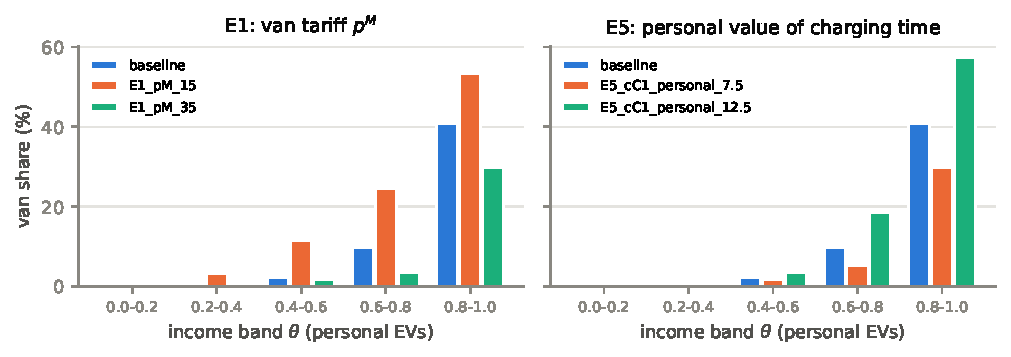
\includegraphics[width=0.95\textwidth]{figures/exp_income.pdf}
\caption{Personal van share by income band (MILP): E1 (van tariff) and E5 (personal value of charging time).}
\label{fig:expincome}
\end{figure}

\begin{itemize}
  \item \textbf{No premium ($p^M=15$)}: $Z$ $-4.2$\,\%. Customers save 7.8\,\%, the operator pays 3.7\,\% more (more vans dispatched, 2.40 instead of 2.17 on average, and dearer van energy). Personal van share 19.8\,\% $\to$ 31.4\,\%; van use spreads down the income scale (Figure~\ref{fig:expincome}: 0.4--0.6 band from 2\,\% to 12\,\%, 0.6--0.8 from 10\,\% to 24\,\%). Commercial van share doubles but stays small (0.7 $\to$ 1.4\,\%).
  \item \textbf{Double premium ($p^M=35$)}: $Z$ $+3.9$\,\%, customers $+6.5$\,\%, operator $-1.4$\,\%. Personal van share falls to 13.5\,\%; even the richest band drops from 41\,\% to 30\,\%.
  \item \textbf{Who gains from cheaper vans}: mostly rich private owners (their felt cost in the top band falls from about Rs 646 to 547), because they are the ones who switch. Poor drivers gain little (Rs 607 to 576), mostly because the stations get less crowded.
  \item 4 instances lose their plan at $p^M=15$ and 3 gain one at $p^M=35$: with more van use the 300-second search gets harder, not the problem itself.
\end{itemize}

\inshort{The van price is the operator's main tool to decide how many and which customers get vans; making vans cheaper mostly helps rich private owners.}

\subsection{E2: van fleet and seats}

\begin{table}[H]
\centering
\caption{E2. 3 or 7 vans (baseline 5); 4 or 8 cars per van (baseline 6).}
\scriptsize
\begin{adjustbox}{max width=\linewidth}
\begin{tabular}{@{}lrrrrrrrrrrr@{}}
\toprule
method & valid & paired & new & lost & \shortstack{$\Delta Z$\\\%} & \shortstack{$\Delta$\\oper. \%} & \shortstack{$\Delta$\\cust. \%} & \shortstack{van \%\\personal} & van \% comm. & vans used & \shortstack{gap to\\MILP \%} \\
\midrule
\multicolumn{12}{@{}l}{\textbf{E2\_vans\_3}: 3 vans} \\
MILP & 441 & 441 & 0 & 33 & $-$0.04 & $-$0.53 & $+$0.20 & 19.4 $\to$ 17.4 & 0.2 $\to$ 0.1 & 1.96 & -- \\
RL zero-shot & 465 & 465 & 0 & 35 & $+$0.02 & $-$0.27 & $+$0.15 & 6.4 $\to$ 5.7 & 0.3 $\to$ 0.2 & 2.00 & 0.91 \\
RL retrained & 466 & 466 & 0 & 34 & $+$0.09 & $-$0.12 & $+$0.18 & 6.4 $\to$ 5.9 & 0.4 $\to$ 0.2 & 2.02 & 0.96 \\
\multicolumn{12}{@{}l}{\textbf{E2\_vans\_7}: 7 vans} \\
MILP & 487 & 474 & 13 & 0 & $+$0.02 & $+$0.22 & $-$0.05 & 19.9 $\to$ 20.5 & 0.7 $\to$ 0.7 & 2.22 & -- \\
RL zero-shot & 506 & 500 & 6 & 0 & $+$0.04 & $+$0.13 & $+$0.03 & 6.7 $\to$ 6.7 & 0.9 $\to$ 1.0 & 2.23 & 0.84 \\
RL retrained & 506 & 500 & 6 & 0 & $+$0.00 & $+$0.06 & $-$0.00 & 6.7 $\to$ 7.0 & 0.9 $\to$ 0.7 & 2.23 & 0.81 \\
\multicolumn{12}{@{}l}{\textbf{E2\_seats\_4}: 4 EVs per van} \\
MILP & 471 & 467 & 4 & 7 & $+$1.08 & $+$3.03 & $+$0.26 & 19.8 $\to$ 11.6 & 0.3 $\to$ 0.2 & 2.48 & -- \\
RL zero-shot & 493 & 493 & 0 & 7 & $+$0.91 & $+$3.87 & $-$0.35 & 6.7 $\to$ 5.8 & 0.5 $\to$ 0.4 & 2.54 & 0.69 \\
RL retrained & 494 & 494 & 0 & 6 & $+$0.88 & $+$4.04 & $-$0.46 & 6.8 $\to$ 7.2 & 0.5 $\to$ 0.3 & 2.55 & 0.65 \\
\multicolumn{12}{@{}l}{\textbf{E2\_seats\_8}: 8 EVs per van} \\
MILP & 471 & 471 & 0 & 3 & $-$0.08 & $-$0.28 & $+$0.06 & 19.9 $\to$ 21.6 & 0.7 $\to$ 0.8 & 2.13 & -- \\
RL zero-shot & 500 & 499 & 1 & 1 & $-$0.08 & $-$0.61 & $+$0.16 & 6.7 $\to$ 6.6 & 0.9 $\to$ 0.9 & 2.13 & 0.85 \\
RL retrained & 499 & 499 & 0 & 1 & $+$0.07 & $-$0.31 & $+$0.25 & 6.7 $\to$ 7.2 & 0.9 $\to$ 0.9 & 2.16 & 0.98 \\
\bottomrule
\end{tabular}
\end{adjustbox}

\end{table}

\begin{itemize}
  \item \textbf{The number of vans does not change the cost} of solvable instances: on the instances optimal in both runs the change is 0.000\,\% for 3 and for 7 vans (Table~\ref{tab:direction}). The plans use only about 2.2 vans on average, so the fifth van is rarely needed for cost.
  \item \textbf{But the number of vans decides feasibility}: with 3 vans 33 instances lose their plan (3 become provably infeasible), with 7 vans 13 new instances get one. These are mostly large R1/RC1 instances (23 of the 33 lost, 10 of the 13 gained; all with 50 or more cars), where stranded cars and late requests need many van trips in a short period. The small changes in the table ($-0.04$\,\%, $+0.02$\,\%) come from time-limited plans, not from a real effect.
  \item \textbf{Fewer seats per van cost money}: with 4 seats $Z$ rises 1.1\,\% (1.3\,\% at the optima), the operator's cost 3.0\,\%: more vans must be dispatched (2.48 instead of about 2.2) to serve the same cars, and the personal van share falls from 19.8 to 11.6\,\%. With 8 seats $Z$ falls only 0.1\,\%: 6 seats are rarely all used.
\end{itemize}

\inshort{More vans buy feasibility in the hardest instances, not lower cost; seats per van matter for cost only when they are cut below the baseline.}

\subsection{E8: van battery}

\begin{table}[H]
\centering
\caption{E8. Van battery 200 kWh instead of 150.}
\scriptsize
\begin{adjustbox}{max width=\linewidth}
\begin{tabular}{@{}lrrrrrrrrrrr@{}}
\toprule
method & valid & paired & new & lost & \shortstack{$\Delta Z$\\\%} & \shortstack{$\Delta$\\oper. \%} & \shortstack{$\Delta$\\cust. \%} & \shortstack{van \%\\personal} & van \% comm. & vans used & \shortstack{gap to\\MILP \%} \\
\midrule
\multicolumn{12}{@{}l}{\textbf{E8\_battery\_200}: B = 200 kWh} \\
MILP & 476 & 473 & 3 & 1 & $-$0.01 & $-$0.40 & $+$0.19 & 19.9 $\to$ 18.5 & 0.7 $\to$ 0.7 & 2.14 & -- \\
RL zero-shot & 501 & 500 & 1 & 0 & $-$0.02 & $-$0.17 & $+$0.05 & 6.7 $\to$ 6.5 & 0.9 $\to$ 0.9 & 2.19 & 0.83 \\
RL retrained & 500 & 499 & 1 & 1 & $-$0.07 & $-$0.06 & $-$0.07 & 6.7 $\to$ 8.2 & 0.9 $\to$ 0.7 & 2.18 & 0.77 \\
\bottomrule
\end{tabular}
\end{adjustbox}

\end{table}

$Z$ changes by $-0.01$\,\% on average ($-0.04$\,\% at the optima). The battery almost never limits a van: seats and time run out first. By the decision rule fixed before the run (less than 1\,\%), \textbf{van recharging need not be modelled}.

\inshort{A bigger battery changes nothing; recharging vans can be left out of the model.}

%=====================================================================
\section{A check of the MILP results against theory}
\label{sec:direction}

Some directions are certain from the model alone. A dearer van tariff can never make the \emph{optimal} cost lower (every plan gets dearer or stays the same); more vans, seats or battery can never make it higher (every old plan is still allowed). On the instances that are \emph{optimal in both} runs, every variant must therefore move $Z$ the right way:

\begin{table}[H]
\centering
\caption{Direction check on instances proven optimal in both the baseline and the variant.}
\label{tab:direction}
\footnotesize
\begin{adjustbox}{max width=\linewidth}
\begin{tabular}{@{}lrrrr@{}}
\toprule
variant & $Z$ at the optimum & optimal in both & mean $\Delta Z$ (\%) & wrong direction \\
\midrule
E1\_pM\_15 & must not rise & 225 & $-$4.448 & 0 \\
E1\_pM\_35 & must not fall & 276 & $+$4.069 & 0 \\
E5\_cC1\_personal\_7.5 & must not rise & 275 & $-$2.190 & 0 \\
E5\_cC1\_personal\_12.5 & must not fall & 252 & $+$1.951 & 0 \\
E5\_omega1\_commercial\_4.5 & must not rise & 275 & $-$2.506 & 0 \\
E5\_omega1\_commercial\_7.5 & must not fall & 275 & $+$2.496 & 0 \\
E6\_mu0\_personal\_1.125 & must not rise & 273 & $-$1.298 & 0 \\
E6\_mu0\_personal\_1.875 & must not fall & 276 & $+$1.299 & 0 \\
E6\_mu0\_commercial\_1.125 & must not rise & 272 & $-$6.449 & 0 \\
E6\_mu0\_commercial\_1.875 & must not fall & 275 & $+$6.457 & 0 \\
E2\_vans\_3 & must not fall & 275 & $+$0.000 & 0 \\
E2\_vans\_7 & must not rise & 273 & $-$0.000 & 0 \\
E2\_seats\_4 & must not fall & 275 & $+$1.297 & 0 \\
E2\_seats\_8 & must not rise & 263 & $-$0.156 & 0 \\
E8\_battery\_200 & must not rise & 274 & $-$0.036 & 0 \\
\bottomrule
\end{tabular}
\end{adjustbox}

\end{table}

\textbf{All 15 variants pass, with \fdirectionBad{} violations} in about 4\,000 pairs of optimal plans. This is a strong sign that the model, the data changes and the solver runs are consistent.

\inshort{Wherever the MILP proved optimality, every experiment moved the cost in the direction the model requires: the results can be trusted.}

%=====================================================================
\section{Which assumption matters most}

\begin{figure}[H]
\centering
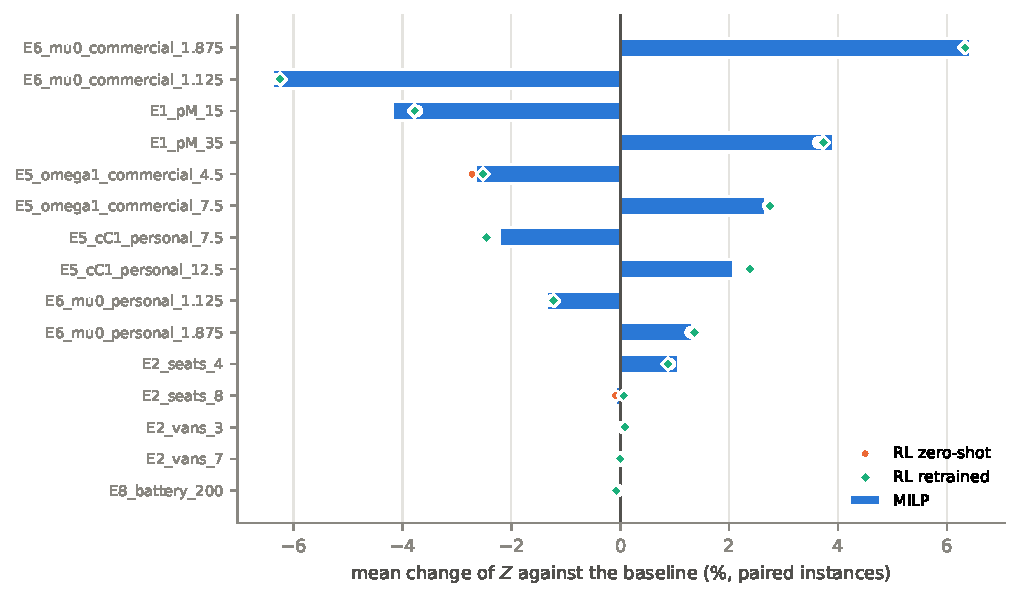
\includegraphics[width=0.9\textwidth]{figures/exp_tornado.pdf}
\caption{Mean change of $Z$ for every variant (bars: MILP; markers: RL, Part V). Sorted by size.}
\label{fig:tornado}
\end{figure}

Ranking by the effect on $Z$ of a $\pm25$\,\% or comparable change:
\begin{enumerate}
  \item commercial money sensitivity $\mu^0$: $\pm6.4$\,\%;
  \item van tariff $p^M$: $-4.2$ / $+3.9$\,\%;
  \item commercial downtime rate $\omega^1$: $\pm2.7$\,\%;
  \item personal value of station time $c^{C,1}$: $\pm2.1$\,\%;
  \item personal money sensitivity $\mu^0$: $\pm1.3$\,\%;
  \item seats per van (only when cut): $+1.1$\,\%;
  \item number of vans, battery: about 0\,\% (but the fleet decides feasibility).
\end{enumerate}
For \emph{who gets vans}, the ranking is different: the van tariff, the personal value of station time and cutting seats move the personal van share by about 6 to 12 percentage points; the money sensitivities and the commercial downtime rate move it by about 1 point or less.

\inshort{To estimate the cost well, measure how poor drivers feel money; to decide who gets vans, set the van tariff and know how much private owners value station time.}
